
\section*{Basic Element}

    Now, we have idea of what neural networks \textbf{are}. But, we have yet to handle the \textbf{details}:
    
    \begin{itemize}
        \item What \textbf{is} a neuron?
        \item How do we "systematically" \textbf{combine} our neurons?
        \item How do we \textbf{train} this, like we would a \textbf{simple} model?
    \end{itemize}
    
    We'll handle all of these steps and more - the above description was just to give a \textbf{high-level} view of what we want to \textbf{accomplish}. 
    
    Now, we go down to the \textbf{bottom} level, and think about just \textbf{one neuron}: what does it look like, and how does it work?
    
    First, some terminology:\\
    
    \begin{notation}
        \vocab{Neurons} are also sometimes called \vocab{units} or \vocab{nodes}.
        
        They are mostly \gren{equivalent} names. They just reflect different \purp{perspectives}.
    \end{notation}
    
    \subsection*{What's in a neuron: The Linear Component}
    
        As we mentioned before, our goal is to combine \textbf{simple} units into a \textbf{bigger} one. So, we want a model that's \textbf{simple}.
        
        Well, let's start with what we've done before: we've worked with the \textbf{linear} model
        
        \begin{equation}
            h(x) = \theta^T x + \theta_0
        \end{equation}
        
        This model has lots of nice properties:
        
        \begin{itemize}
            \item It limits itself to \textbf{addition} and \textbf{multiplication} (easy to compute)
            
            \item \textbf{Linearity} lets us prove some mathematical things, and use vector/\textbf{matrix} math
            
            \item The dot product between $\theta$ and $x$ has a nice \textbf{geometric} interpretation.
        \end{itemize}
        
        This will make up the \textbf{first} part of our model.\\
        
        \begin{concept}
            Our \vocab{neuron} contains a \purp{linear} function as its \gren{first} component.
        \end{concept}
    
    \subsection*{Weights and Biases}
    
        But, there's one minor \textbf{change}: before, we used $\theta$ because it represented our \textbf{hypothesis}. 
        
        But, every neuron is going to have its own \textbf{values} for its \textbf{linear} model:
        
        \begin{equation}
            \overbrace{
                f_1(x)
            }^{\text{Neuron 1}}
            = Ax+B 
            \qquad \qquad \qquad
            \overbrace{
                f_1(x)
            }^{\text{Neuron 2}}
            = Cx+D
        \end{equation}
        
        It wouldn't make much \textbf{sense} to call both $A$ and $C$ by the name $\theta$. 
        
        We could use some clever \textbf{notation}, but why treat them as \textbf{hypotheses}? They are each only a \textbf{part} of our hypothesis $\Theta$.
        
        So, instead of thinking of each as a "hypothesis", let's switch perspectives.
        
        Each value $\theta_k$ \textbf{scales} how much $x_k$ affects the \textbf{output}: if we're doing
        
        \begin{equation}
            g(x) = 100x_1+2x_2
        \end{equation}
        
        Then, changing $x_1$ will have a much \textbf{bigger} effect on $g(x)$. Another way to say this is it \textbf{weighs} more heavily: it matters \textbf{more}.
        
        Because of that, we call the number we scale $x_1$ by a \textbf{weight}.\\
        
        \begin{notation}
            A \vocab{weight} $w_k$ tells you how heavily a \purp{variable} $x_k$ \gren{weighs} into the output.
            
            $w_k$ is \purp{equivalent} to $\theta_k$: it's a \gren{scalar} $w_k \in \RR$.
            
            \begin{equation*}
                \Big( 
                    \red{\theta_1}x_1 + \blu{\theta_2}x_2 
                \Big)
                \Longleftrightarrow 
                \Big(
                    \red{w_1}x_1+\blu{w_2}x_2
                \Big)
            \end{equation*}
            
            We can combine it into a vector $w \in \RR^m$.
            
            \begin{equation*}
                w = 
                    \begin{bmatrix}
                      w_1 \\ w_2 \\ \vdots \\ w_m
                    \end{bmatrix}
                \qquad \qquad \qquad
                \theta^Tx \Longleftrightarrow w^Tx
            \end{equation*}
        \end{notation}
        
            \note{Remember that $a \Longleftrightarrow b$ means $a$ and $b$ are equivalent!} 
        
        
        What about our other term, $\theta_0$? We call it an \textbf{offset}: it's the value we \textbf{shift} our linear model away from \textbf{origin}.
        
        We'll use the same notation:\\
        
        \begin{notation}
            An \vocab{offset} $w_0$ tells you how far we \purp{shift} $h(x)$ away from the origin. 
            
            $w_0$ is \purp{equivalent} to $\theta_0$: it's a \gren{scalar} $w_0 \in \RR$
            
            \begin{equation*}
                \Big(
                    (\theta^Tx) + \red{\theta_0} 
                \Big)
                \Longleftrightarrow 
                \Big(
                    (w^Tx) + \red{w_0}
                \Big)
            \end{equation*}
            
            We also sometimes call this the \vocab{threshold} or the \vocab{bias}.
            
            Alternate notation: we might call this variable $\red{b}$, for bias.
        \end{notation}
        
        This gives us our linear model using our new notation:\\
        
        \begin{definition}
            The \vocab{linear component} for a neuron is given by
            
            \begin{equation*}
                z(x) = w^Tx + w_0
            \end{equation*}
            
            where $w \in \RR^m$ and $w_0 \in \RR$.
            
            \begin{equation*}
                w = 
                    \begin{bmatrix}
                      w_1 \\ w_2 \\ \vdots \\ w_m
                    \end{bmatrix}
            \end{equation*}
        \end{definition}
    
    \subsection*{Linear Diagram}
    
        Now, we want to be able to depict our \textbf{linear} subunit. Let's do it piece-by-piece.
        
        First, we have our vector $\blu{x} = [x_1, x_2, ..., x_m]^T$:
        
        \begin{figure}[H]
            \centering
            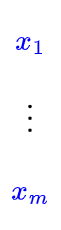
\includegraphics[width=10mm,scale=0.4]{images/nn_images/x_vector.png}
        \end{figure}
        
        Now, we want to \textbf{multiply} each term $x_i$ by its corresponding \textbf{weight} $w_i$. We'll combine them into a \textbf{function}:
        
        
        \begin{figure}[H]
            \centering
            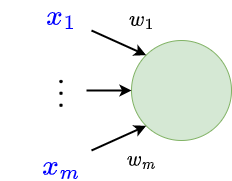
\includegraphics[width=30mm,scale=0.4]{images/nn_images/weights.png}
            \caption*{The circle represents our function.}
        \end{figure}
        
        How are we combining them? Well, we're adding them together.
        
        \begin{figure}[H]
            \centering
            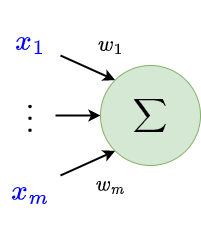
\includegraphics[width=25mm,scale=0.4]{images/nn_images/sigma.png}
        \end{figure}
        
        Note that we use the $\sum$ symbol, because we're \textbf{adding} after we \textbf{multiply}. In fact, we can write this as
        
        \begin{equation}
            w^T \blu{x} = \sum_{i=1}^m w_i\blu{x_i}
        \end{equation}
        
        We'll include the bias term as well: remember that we can represent $w_0$ as $1 * w_0$ to match with the other terms.
        
        \begin{figure}[H]
            \centering
            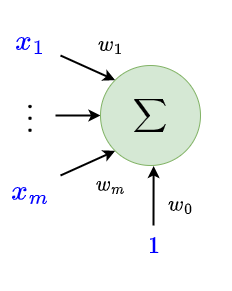
\includegraphics[width=30mm,scale=0.4]{images/nn_images/bias.png}
            \caption*{The blue "1" term is \textbf{multiplied} by $w_0$, just like how $x_k$ gets multiplied by $w_k$.}
        \end{figure}
        
        We have our full function! All we need to do is include our output, $\red{z}$:\\
        
        \begin{notation}
            We can depict our linear function $\red{z} = w^T\blu{x}+w_0$ as
            \begin{figure}[H]
            \centering
            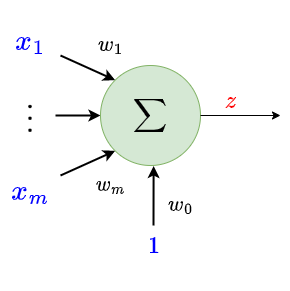
\includegraphics[width=40mm,scale=0.4]{images/nn_images/linear_subunit.png}
        \end{figure}
        \end{notation}
        
        Thus, $z$ is a function of $x$:
        
        \begin{equation}
            \red{z}(\blu{x}) = w^T\blu{x}+w_0
        \end{equation}
        
        Which, in $\sum$ notation, we could write as
        
        \begin{equation}
            \red{z}(\blu{x}) = \Bigg( \sum_{i=1}^m w_i\blu{x_i} \Bigg) +w_0
        \end{equation}
        
    \subsection*{Adding nonlinearity}
    
        We'll continue building our neuron based on what we've done \textbf{before}. When doing linear regression, that linear unit was all we had. 
        
        But, once we do classification, we found that it was helpful to have a second, \textbf{non-linear} component: we used \textbf{sigmoid} $\sigma(u)$.
        
        We might not necessarily want the \textbf{same} nonlinear function, so instead, we'll just generalize: we have \textit{some} second component, which is allowed to be \textbf{nonlinear}.
        
        We call this component our \textbf{activation} function. Why do we call it that? It comes from the historical \textbf{inspiration} of neurons in the brain.
        
        Biological neurons only "fire" (give an output) above a certain threshold of \textbf{input}: that's when they \textbf{activate}.
            \note{Some activation functions reflect this, but they don't have to.}\\
            
        \begin{definition}
            Our \vocab{neuron} contains a potentially \purp{nonlinear} function $f$ called an \vocab{activation function} as its \gren{second} component.
            
            We notate this as 
            
            \begin{equation}
                \pur{a} = f(\red{z})
            \end{equation}
            
            Where $z$ is the \gren{output} of the \purp{linear} component, and $a$ is the \gren{output} of the \purp{activation} component.
            
            Note that $z$ and $a$ are \purp{real numbers}: we have $f: \RR \rightarrow \RR$
            
        \end{definition}
    
    \subsection*{Nonlinear Diagram}
    
        We'll depict a function $f$.

        \begin{figure}[H]
            \centering
            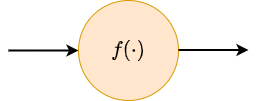
\includegraphics[width=40mm,scale=0.4]{images/nn_images/nonlinear_func.png}
        \end{figure}
        
        It takes in our \textbf{linear} output, $\red{z}$, and outputs our \textbf{neuron} output, $\pur{a}$.
        
        \begin{figure}[H]
            \centering
            \qquad\quad\;
            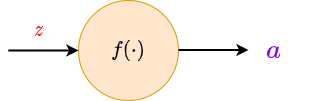
\includegraphics[width=60mm,scale=0.4]{images/nn_images/nonlinear_unit.png}
        \end{figure}
        
        Note some vocabulary used for $z$:\\
        
        \begin{notation}
            $z$, the \purp{output} of our \gren{linear} function, is called the \vocab{pre-activation}.
            
            This is because it is the result \purp{before} we run the \gren{activation} function.
        \end{notation}
        
        And for $a$:\\

        \begin{notation}
            $a$, the \purp{output} of our \gren{activation} function, is called the \vocab{activation}.
        \end{notation}
        
    \subsection*{Putting it together}
    
        So now, our neuron is complete.\\

        \begin{definition}
            Our \vocab{neuron} is made of 
            
            \begin{itemize}
                \item A \vocab{linear} component that takes the neuron's input \blu{$x$}, and applies a linear function  
                
                    \begin{equation*}
                        \red{z} = w^T \blu{x} + w_0
                    \end{equation*}
                    
                    \begin{itemize}
                        \item The \vocab{pre-activation} $\red{z}$ is the \purp{output} of the \purp{linear} function.
                        \item It is also the \gren{input} of the \gren{activation function} $f$.
                    \end{itemize}
                    
                \item A (potentially nonlinear) \vocab{activation} component that takes the pre-activation $\red{z}$ and applies an \vocab{activation function} $f$:
                
                    \begin{equation*}
                        \pur{a} = f(\red{z})
                    \end{equation*}
                    
                    \begin{itemize}
                        \item The \vocab{activation} $\pur{a}$ is the \purp{output} of this \purp{activation function}.
                    \end{itemize}
            \end{itemize}
            
            When we \purp{compose} them together, we get
            
            \begin{equation*}
                \pur{a} = f(\red{z}) = f \Big(  w^T \blu{x} + w_0 \Big)
            \end{equation*}
            
        \end{definition}
        
            \note{When we say "compose", we mean \textbf{function composition}: combining $f(x)$ and $g(x)$ into $f(g(x))$.}
        
        We can also use $\sum$ notation to get:
        
        \begin{equation*}
            \pur{a} = f(\red{z}) = 
            f 
            \Bigg(
                \bigg( 
                    \sum_{i=1}^m w_i\blu{x_i} 
                \bigg) 
                + w_0 
            \Bigg)
        \end{equation*}
        
    \subsection*{Neuron Diagram}
    
        Finally, we can \textbf{compose} our neuron into one big \textbf{diagram}:
        
        \begin{figure}[H]
            \centering
            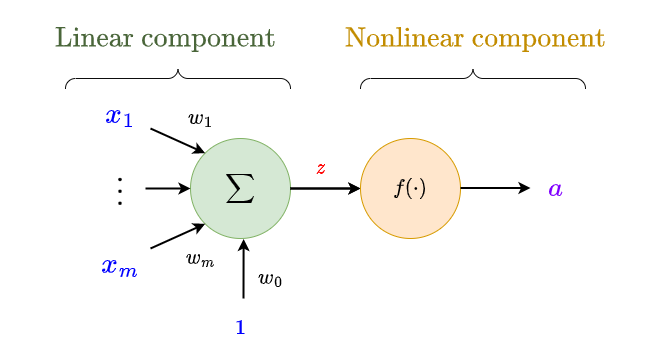
\includegraphics[width=100mm,scale=0.4]{images/nn_images/labelled_neuron.png}
        \end{figure}
        
        From here on out, we'll treat this as a \textbf{single} object:
        
        \begin{figure}[H]
            \centering
            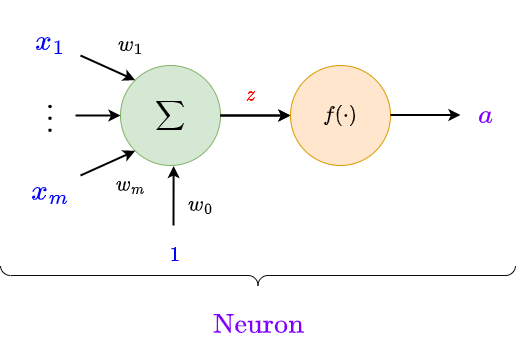
\includegraphics[width=80mm,scale=0.4]{images/nn_images/neuron_underbrace.png}
        \end{figure}
        
        \begin{notation}
            We can depict our \vocab{neuron} $f(w^T\blu{x}+w_0)$ as
            
            \begin{figure}[H]
                \centering
                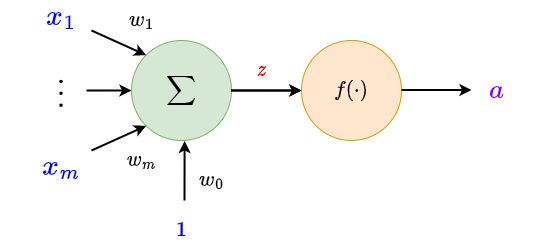
\includegraphics[width=100mm,scale=0.4]{images/nn_images/full_neuron.png}
            \end{figure}
            
            \begin{itemize}
                \item $x$ is our \gren{input} (neuron input, linear input )
                
                \item $z$ is our \purp{pre-activation} (linear output, activation input)
                
                \item $a$ is our \purp{activation} (neuron output, activation output)
            \end{itemize}
        \end{notation}
    
        This neuron will be the \textbf{basic unit} we work with for the rest of this \textbf{chapter} - it's one of the most \textbf{important} objects in all of machine learning.
        
    \subsection*{Our Loss Function}
    
        One more detail: we will want to \textbf{train} these neurons. In order to be able to \textbf{measure} their performance, we'll need a \textbf{loss} function.
        
        This \textbf{isn't} any different from usual: we just need a \textbf{function} of the form
        
        \begin{equation}
            \loss(g,y)
        \end{equation}
        
        In \textbf{regression}, we wrote our loss as
        
        \begin{equation*}
            \loss 
            \Big( \;\;
                \blu{h(x; \Theta)}, \;\;
                \red{y} 
            \;\;\Big) 
        \end{equation*}
        
        The right term, $\eyi$, is unchanged: we still need to compare against the \textbf{correct} answer.
        
        The main change is we aren't using $\Theta$ notation: we'll \textbf{replace} it with $(w,w_0)$
        
        \begin{equation*}
            \loss 
            \Bigg( \;\;
                h
                \Big(
                    x; \pur{(w, w_0)}
                \Big), \;\;
                y 
            \;\;\Bigg) 
        \end{equation*}
        
        And finally, we get the loss for multiple data points: 
            \note{We skip doing $1/n$ averaging because we often use this for SGD: we plan to take small steps as we go, rather than adding up our steps all at once.}
        \begin{equation*}
            \sum_i
            \loss 
            \Bigg( \;\;
                h
                \Big(
                    \blu{\exi}; (w, w_0)
                \Big), \;\;
                \blu{\eyi} 
            \;\;\Bigg) 
        \end{equation*}
        
        And with this, not only is our neuron \textbf{complete}, but we have everything we need to \textbf{work} with it.\\
        
        \begin{concept}
            For a \vocab{complete neuron}, we need to specify
        
            \begin{itemize}
                \item Our \purp{weights} and \gren{offset}
                \item Our \purp{activation} function
                \item Our \purp{loss} function
            \end{itemize}
        \end{concept}
        
        From here, we could do \textbf{stochastic gradient descent} as we usually do, to \textbf{optimize} this neuron's \textbf{performance}.
        